\documentclass[8pt,a4paper,compress]{beamer}

\usepackage{/home/siyer/lib/slides}

\title{Balanced Search Trees}
\date{}

\begin{document}
\begin{frame}
\vfill
\titlepage
\end{frame}

\begin{frame}
\frametitle{Outline}
\tableofcontents
\end{frame}

\section{2-3 Search Trees}
\begin{frame}[fragile]
\begin{itemize}
\item a 2-3 search tree is a tree that is either empty (null link) or
\begin{itemize}
\item a 2-node with one key (and associated value) and two links, a left link to a 2-3 search tree with smaller keys, and a right link to a 2-3 search tree with larger keys

\item a 3-node with two keys (and associated values) and three links, a left link to a 2-3 search tree with smaller keys, a middle link to a 2-3 search tree with keys between the node's keys, and a right link to a 2-3 search tree with larger keys
\end{itemize}

\begin{center}
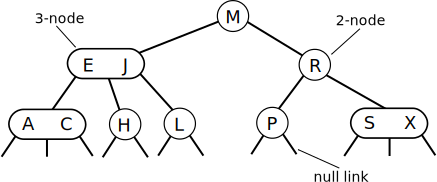
\includegraphics[scale=0.4]{{./figures/23_tree}.png}
\end{center}

\item a 2-3 search tree has symmetric order --- inorder traversal yields keys in ascending order

\item a perfectly balanced 2-3 search tree is one whose null links are all the same distance from the root

\begin{center}
\includegraphics[scale=0.3]{{./figures/23_tree_perfect_balance}.png}
\end{center}
\end{itemize}
\end{frame}

\begin{frame}[fragile]
\begin{itemize}
\item searching for a key in a 2-3 tree
\begin{center}
\includegraphics[scale=0.4]{{./figures/23_tree_search}.png}

\smallskip

search hit (left) and search miss (right) in a 2-3 tree
\end{center}
\end{itemize}
\end{frame}

\begin{frame}[fragile]
\begin{itemize}
\item inserting into a 2-3 tree
\begin{itemize}
\item insert into a 2-node
\begin{center}
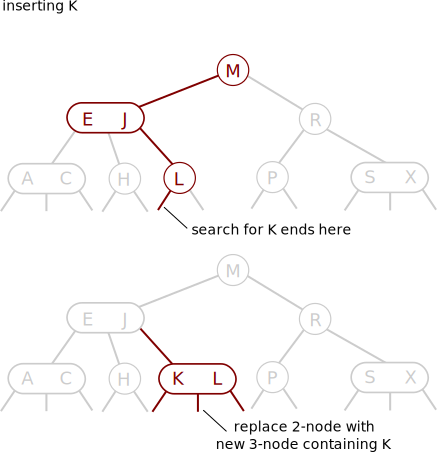
\includegraphics[scale=0.4]{{./figures/23_tree_insert1}.png}
\end{center}

\item insert into a single 3-node
\begin{center}
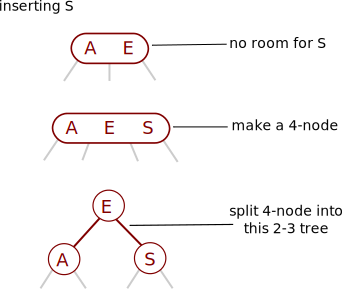
\includegraphics[scale=0.4]{{./figures/23_tree_insert2}.png}
\end{center}
\end{itemize}
\end{itemize}
\end{frame}

\begin{frame}[fragile]
\begin{itemize}
\item inserting into a 2-3 tree (contd.)
\begin{itemize}
\item insert into a 3-node whose parent is a 2-node
\begin{center}
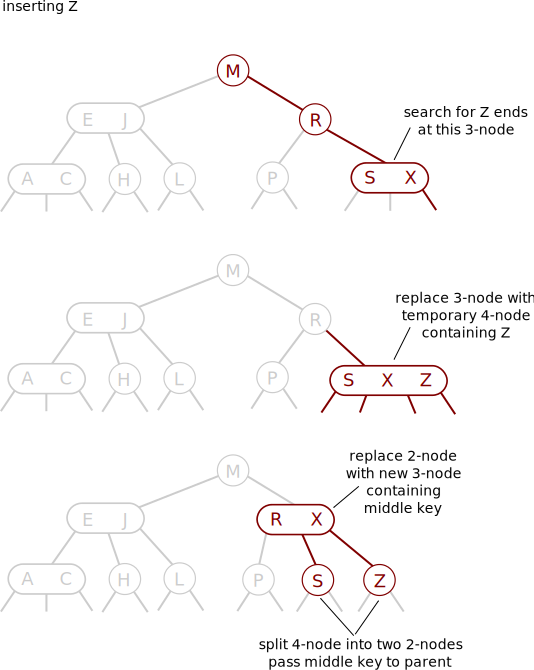
\includegraphics[scale=0.4]{{./figures/23_tree_insert3}.png}
\end{center}
\end{itemize}
\end{itemize}
\end{frame}

\begin{frame}[fragile]
\begin{itemize}
\item inserting into a 2-3 tree (contd.)
\begin{itemize}
\item insert into a 3-node whose parent is a 3-node
\begin{center}
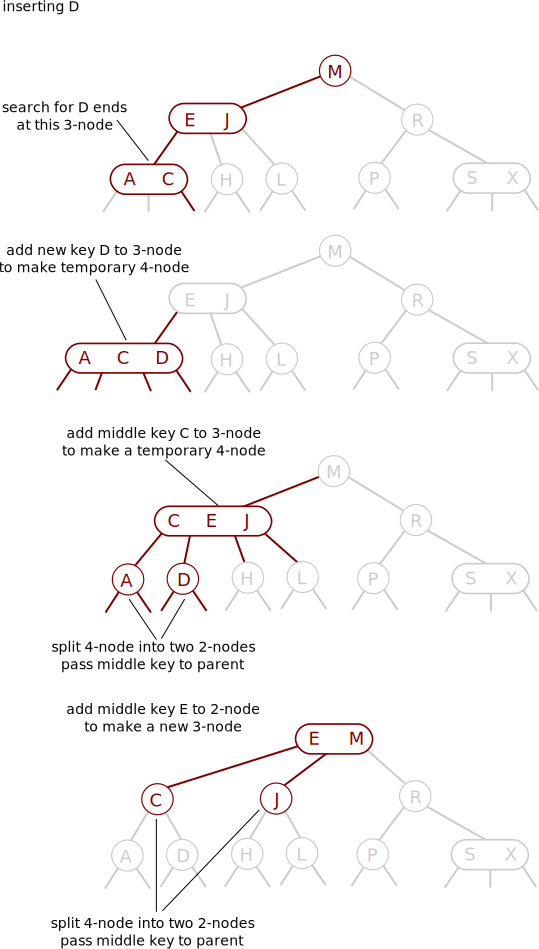
\includegraphics[scale=0.4]{{./figures/23_tree_insert4}.png}
\end{center}
\end{itemize}
\end{itemize}
\end{frame}

\begin{frame}[fragile]
\begin{itemize}
\item inserting into a 2-3 tree (contd.)
\begin{itemize}
\item splitting the root
\begin{center}
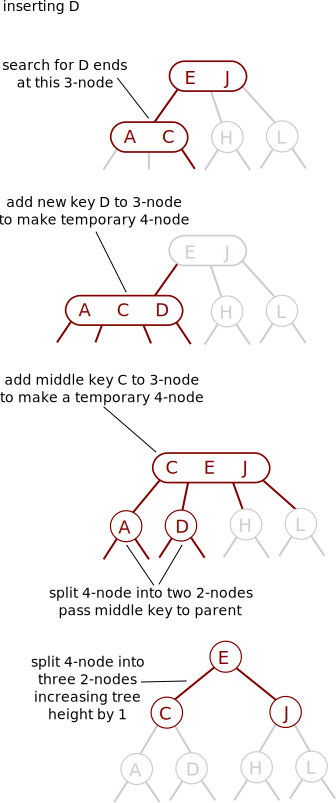
\includegraphics[scale=0.4]{{./figures/23_tree_insert5}.png}
\end{center}
\end{itemize}
\end{itemize}
\end{frame}

\begin{frame}[fragile]
\begin{itemize}
\item splitting a 4-node is a local transformation: constant number of operations

\item insert operation maintains symmetric order and perfect balance

\item tree height
\begin{itemize}
\item worst case: $\lg N$ (all 2-nodes)

\item best case: $\log_3 N \approx 0.631 \lg N$ (all 3-nodes)

\item between 12 and 20 for a million nodes

\item between 18 and 30 for a billion nodes
\end{itemize}

\item guaranteed logarithmic performance for search and insert
\end{itemize}
\end{frame}

\begin{frame}[fragile]
\begin{itemize}
\item direct implementation is complicated because:
\begin{itemize}
\item maintaining multiple node types is cumbersome

\item need multiple comparisons to move down tree

\item need to move back up the tree to split 4-nodes

\item large number of cases for splitting
\end{itemize}

\smallskip

fantasy code:
\begin{lstlisting}[language=Java]
public void put(Key key, Value val) {
    Node x = root;
    while (x.getTheCorrectChild(key) != null) {
        x = x.getTheCorrectChildKey();
        if (x.is4Node()) { x.split(); }
    }
    if (x.is2Node()) { x.make3Node(key, val); }
    else if (x.is3Node()) { x.make4Node(key, val); }
}
\end{lstlisting}

could do it, but there's a better way (use red-black BSTs)
\end{itemize}
\end{frame}

\section{Red-Black BSTs}
\begin{frame}[fragile]
\begin{itemize}
\item 
\end{itemize}
\end{frame}

\section{B-Trees}
\begin{frame}[fragile]
\begin{itemize}
\item 
\end{itemize}
\end{frame}

\end{document}
